\documentclass[addpoints]{exam}

\usepackage{graphbox}
\usepackage{hyperref}
\usepackage{listings}
\usepackage{tabularx}
\usepackage{tikz}
\usetikzlibrary{positioning}

% Header and footer.
\pagestyle{headandfoot}
\runningheadrule
\runningfootrule
\runningheader{CS 440}{HW 1: Math \& JS}{Fall 2019}
\runningfooter{}{Page \thepage\ of \numpages}{}
\firstpageheader{}{}{}

% \qformat{{\large\bf \thequestion. \thequestiontitle}\hfill[\totalpoints\ points]}
\qformat{{\large\bf \thequestion. \thequestiontitle}\hfill}
\boxedpoints
% \printanswers

\title{Homework 1: Math and JavaScript}
\author{CS 440 Computer Graphics\\Habib University\\Fall 2019}
% \date{\numpoints\ points, Due: 18h on Wednesday, 11 September}
\date{Due: 18h on Wednesday, 11 September}

\begin{document}
\maketitle

Each problem below specifies the names of the files you have to submit for it. Please make sure your submitted files have the indicated names. Any files in your GitHub repository with these names at the time of the deadline will be considered to be your submission.

\begin{questions}

  \titledquestion{Geometry trumps JS}[0]

  We will be using WebGL to render 3D geometry in the browser. Programming for WebGL is done in JavaScript which is not natively aware of geometric types, e.g. vector or matrix. The file, \texttt{MV.js}, in the \texttt{Common} folder in the \texttt{Code} section on the \href{https://www.cs.unm.edu/~angel/BOOK/INTERACTIVE_COMPUTER_GRAPHICS/SEVENTH_EDITION/}{website of Module I's book} defines abstractions that allow programs to be written in terms of geometric entities, e.g. vectors, instead of JavaScript arrays. It also defines a function to convert these abstract data types to the required JavaScript types when needed. Using this file, we can write code in terms of constructs that are more natural to our application domain

  Go over the file {\tt MV.js} in order to get familiar with the types that it provides and their related operations. You need not spend too much time understanding the function bodies as long as you can infer, e.g. from its name, what the function does. For now, you may skip the functions in the following sections in the file.
  \begin{itemize}
  \item Basic Transformation Matrix Generators, 
  \item ModelView Matrix Generators, and
  \item Projection Matrix Generators.
  \end{itemize}

  Wherever possible in your code for subsequent problems, prefer using geometric primitives and operations from {\tt MV.js} over those provided by JavaScript.
  
  \titledquestion{Taking it for a Spin}[10]

  In this problem we will utilize some of the functionality provided by \texttt{MV.js}. Write a JavaScript script which asks the user for a dimension between 2 and 4 inclusive and then inputs 2 vectors of that dimension. It then presents the user a menu with the following choices.
  \begin{itemize}
  \item Tell whether the vectors are equal
  \item Show the lengths of the vectors
  \item Show the normalized vectors
  \item Show the sum of the vectors
  \item Show the difference of the vectors
  \item Show the dot product of the vectors
  \item Show the cross product of the vectors
  \item Exit
  \end{itemize}
  The program should repeat until the user chooses to exit.

  Use JavaScript and \texttt{MV.js} only. Do not use any higher level library. You may have to look up how to perform user I/O in JavaScript. Output typically uses \texttt{alert()} or \texttt{console.log()}. Make sure to find out how to invoke your browser's \textit{console} as that will often be your only means to debug your program.

  Write your program in 2 files--\texttt{operations.html} and \texttt{operations.js}--where the program logic resides in \texttt{operations.js} and the HTML file includes \texttt{operations.js} and \texttt{MV.js}. Opening the HTML file in a browser should start the program. \\
  \underline{Files}: operations.html, operations.js
  
  \titledquestion{Mapping and Linear Interpolation}[0]
  \label{q:interpolate}

  \begin{tabularx}{\linewidth}{cX}
    \raisebox{-\totalheight}{
      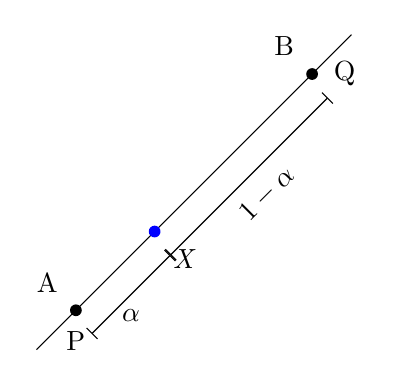
\begin{tikzpicture}
        \draw (0,0) -- (4,4);
        \node[circle,fill,inner sep=1.5pt] at (.5,.5) (P){};
        \node[circle,fill,inner sep=1.5pt] at (3.5,3.5) (Q) {};
        \node[circle,fill,blue,inner sep=1.5pt] at (1.5,1.5) (X) {};
        \node[below  = 2pt of P]{P};
        \node[right = 2pt of Q]{Q};
        \node[below right = 2pt of X]{\it X};
        \node[above left = 2pt of P]{A};
        \node[above left = 2pt of Q]{B};

        \draw[|-|] (0.7,0.2) -- node[midway,below=2pt]{$\alpha$}(1.7,1.2);
        \draw[|-|] (1.7,1.2) -- node[midway,sloped,below=2pt]{$1-\alpha$}(3.7,3.2);
      \end{tikzpicture}
    }
    &
    In the figure on the left, $X$ lies on the line segment $PQ$ such that
    \[
      |PX| : |XQ| = \alpha:(1-\alpha)\;,\; 0 \leq \alpha \leq 1,
    \]
    which leads to
    \[
      X = \alpha Q + (1-\alpha) P.
    \]
    $X$ is thus said to be an \href{https://en.wikipedia.org/wiki/Affine_combination}{\it affine combination} of $P$ and $Q$.
    
    Imagine a mapping from the range $PQ$ to a new range $AB$. Write a function {\tt map\_point} that takes $P$, $Q$, $A$, $B$, and $X$ as parameters and uses the {\tt mix} function from the file {\tt MV.js} to compute and return the mapping of $X$ to the range $AB$. $P$, $Q$, and $X$ are of the same type which may be a scalar or any of the vectors defined in \texttt{MV.js}. $A$ and $B$ are of the same type which may be a scalar or any of the vectors defined in \texttt{MV.js}. Your function should return a value of the same type as $A$ and $B$.
    This function will be useful in this and subsequent assignments.
  \end{tabularx}
  \underline{Files}: map.js
  
  
  \titledquestion{Color Interpolation}
  \label{q:colorbar}.
  
  \begin{center}
    \includegraphics[width=\linewidth]{barbw}\\
    \vspace{-75pt}\includegraphics[width=\linewidth]{barrgb}
  \end{center}

  WebGL renders in a \emph{canvas} in an HTML page. Individual pixels in the canvas have \emph{pixel coordinates} which start at 0 on the left and increase rightward. Pixel coordinates are always whole numbers. WebGL imposes a coordinate system on the canvas in which the origin is at the middle of the canvas, the left and right extremes of the canvas have $x$ values of -1 and 1 respectively, and the bottom and top extremes of the canvas have $y$ values of -1 and 1 respectively. WebGL uses this coordinate system regardless of the actual dimensions of the canvas.

  Imagine interpolating colors as shown above using WebGL. The width of the canvas is equal to $W$ pixels. In the figure on the top, the left extreme of the canvas corresponds to black (\emph{vec3(0,0,0)}) and the rightmost to white (\emph{vec3(1,1,1)}). The pixels between the horizontal extremes are different shades of gray. 

  In the lower figure, the left extreme of the canvas corresponds to red (\emph{vec3(1,0,0)}), the center to green (\emph{vec3(0,1,0)}), and the right extreme to blue (\emph{vec3(0,0,1)}). The pixels between the left and the center have a color value interpolated between red and green. The pixels between the center and the right have a color value interpolated between green and blue.

  Write a script that inputs $W$, the width of the canvas, and a valid pixel coordinate, i.e. $\in [0, W)$, and uses your function from Problem \ref{q:interpolate} to output
  \begin{parts}
    \part the corresponding WebGL coordinate (assume $y$ to be $0$),
    \part the value of the corresponding shade of gray, and
    \part the value of the corresponding color.
  \end{parts}
  \noindent\underline{Files}: {interpolate.html, interpolate.js}


  \titledquestion{The Mandelbrot Set}

  \begin{center}
      \includegraphics[width=.46\linewidth]{mandelbrot1} \includegraphics[width=.46\linewidth]{mandelbrot2}\\
  \end{center}

  Imagine visualizing the \href{http://en.wikipedia.org/wiki/Mandelbrot_set}{Mandelbrot set} as shown above. The Mandelbrot set consists of complex numbers lying in the circle of radius 2 at the origin in the complex plane. The visualizations above show the relevant portion of the complex plane; the top left corner corresponds to $-2+2i$ and the bottom right to $2-2i$. Each pixel in the visualization corresponds to a complex number. The colors assigned to the pixels in the visualizations are based on certain properties of the corresponding complex numbers but they can be ignored for this problem. The canvas in both cases has the same width and height, $L$. As always, WebGL imposes its own coordinate system on the canvas as described in Problem \ref{q:colorbar}.

  Write a script that inputs $L$ and a pixel position defined by its row and column number. In the context of the canvas the origin is at the top left, the column number increases from left to right and the row number increases from top to bottom. Your script should then use your function from Problem \ref{q:interpolate} to output
  \begin{parts}
    \part the complex number corresponding to the input pixel, and
    \part the corresponding WebGL coordinate.
  \end{parts}
  \noindent\underline{Files}: {mandelbrot.html, mandelbrot.js}
  
\end{questions}

\end{document}